% pdf/a 
\begin{filecontents*}[overwrite]{\jobname.xmpdata}
    \Title{Önálló laboratórium 2 dolgozat}
    \Author{Szilágyi Gábor}
    \Language{hu-HU}
    \Subject{Modell-redukció alkalmazása az elektromágneses térszámításban}
    \Keywords{POD}
    \Publisher{Szilágyi Gábor}
\end{filecontents*}

\documentclass[a4paper,12pt,titlepage]{article}
%\documentclass[a4paper,12pt,titlepage,draft]{article}
\usepackage{ucs}
\usepackage[T1]{fontenc}
\usepackage[utf8]{inputenc}
\usepackage[magyar]{babel}
\usepackage{amsfonts}
\usepackage{amsmath,bm}
\usepackage{amssymb}
\usepackage{graphicx}
%\usepackage[hang]{caption}
\usepackage{subcaption}
\usepackage{blkarray,booktabs,bigstrut} % a címkézett mátrixhoz
%\usepackage{enumerate}
%\usepackage{psfrag}
\usepackage[left=25mm,right=25mm,top=25mm,bottom=25mm]{geometry}
%\usepackage[hyphenbreaks]{breakurl}
%\usepackage[hyphens]{url}
%\usepackage{multirow}
%\usepackage{booktabs}
\usepackage{hyperref}
\usepackage{listings}
%\usepackage{cite}
%\usepackage{csquotes}
\usepackage{siunitx}
\usepackage{xcolor}
\usepackage[a-3u]{pdfx}
\hypersetup{
    colorlinks,
%    linkcolor={red!50!black},
    linkcolor={black},
%    citecolor={blue!50!black},
    citecolor={black},
%    urlcolor={blue!80!black}
    urlcolor={blue!80!black}
}

\sisetup{
    range-phrase=--,
    range-units=single,
    output-decimal-marker={,},
    tight-spacing=true,
    print-unity-mantissa=false,
}

\DeclareMathOperator{\rot}{rot}
%\DeclareMathOperator{\min}{min}
\DeclareMathOperator{\divergence}{div}

\sloppy % Margón túllógó sorok tiltása.
\widowpenalty=10000 \clubpenalty=10000 %A fattyú- és árvasorok elkerülése
\def\hyph{-\penalty0\hskip0pt\relax} % Kötőjeles szavak elválasztásának engedélyezése

\frenchspacing
\pagestyle{plain} 

%\listfiles % a package-ek kilistázása a logba

\title{
    \centering
    
\includegraphics[width=0.48\textwidth]{kep/bme_logo.pdf} \\
    \vspace{0.5cm}
    \large{\bf Budapesti Műszaki és Gazdaságtudományi Egyetem \\
    Villamosmérnöki és Informatikai Kar \\
    Szélessávú Hírközlés és Villamosságtan Tanszék}\\
    \vspace{4cm}
    \large{Önálló laboratórium 2 dolgozat} \\
    \vspace{2cm}
    \Large{\bf{Modell-redukció alkalmazása\\ az elektromágneses térszámításban}} \\
    \vspace{2cm}
}

%\parskip=10pt
%\parindent=0pt

\newcommand\adj[1]{#1^{\mathrm{H}}}

\author{Szilágyi Gábor \\\vspace{2cm}\\ Konzulens: Dr. Bilicz Sándor}
\date{Budapest, \today}


\begin{document}
    \maketitle
    \setcounter{page}{2}
    \section{Bevezetés}
            A POD, vagyis a Proper Orthogonal Decomposition, egy bázistranszformációs eljárás, ami egy adott adathalmaz reprezentálásához optimális bázist keres meg. Az eljárás által meghatározott $\Psi$ bázisban a bázisvektoroknak az a tulajdonsága, hogy a lehető legkevesebb bázisvektorral leírható az adathalmaz információtartalmának vagy energiájának lehető legnagyobb része. Ezt felhasználva a $\Psi$ csonkításával egy $\Psi'$ közelítő bázist lehet előállítani, ami lényegesen kisebb rendű, mint $\Psi$, mégis kis hibával reprezentálható benne az eredeti adathalmaz. Természetesen minél több bázisvektort hagyunk meg $\Psi'$-ben, annál jobban csökken a modell-redukcióból származó hiba, de a csonkítás mértékét az adott alkalmazáshoz mérten előírhatjuk. A POD egy másik előnyös tulajdonsága, hogy a gyakorlati esetek nagy részében a sorbarendezett $\Psi_n$ bázisvektorokra eső energiatartalom a legtöbb esetben rohamosan csökken, ezért sokszor nagyságrendekkel kisebb dimenziószámú bázissal is jól leírható az adathalmaz, mint az eredeti esetben.
        \subsection{A módszer eredete}
            A módszer gyökerei az '40-es évekig nyúlnak vissza, amikor olyan tudományos problémákat próbáltak statisztikai módszerekkel megközelíteni, amelyeknek a megoldása valamilyen folytonos értékű függvény, sok esetben sztochasztikus folyamat. Egy jeles személy ebből a kezdeti időszakból Damodar Dharmananda Kosambi indiai matematikus \cite{Kosambi11}, aki a POD alapját képező (Kosambi--)Karhunen–Lo\`eve Expansion, vagyis Karhunen–Lo\`eve felbontás atyja. A Karhunen–Lo\`eve felbontás sztochasztikus folyamatok olyan reprezentálását teszi lehetővé, ahol a sztochasztikus folyamatot egy végtelen összeg alakjában írjuk fel. Ha ebből az összegből csak az első véges sok $n$ számú tényezőt hagyjuk meg (csonkítjuk a felbontást), akkor a kapott összegnek a lehető legkisebb a négyzetes hibája az eredeti sztochasztikus folyamathoz képest \cite{Aadithya18}.
            \par
            A POD klasszikus formájában végtelen dimenziós vektorterek, például függvényterek fölött működik. Valójában numerikusan ennek egy véges dimenziós vektortereken értelmezett megfelelőjét, a szinguláris érték szerinti felbontást (SVD) lehet használni, a féléves munkám során én is ezt az eljárást használtam. A végtelen és véges dimenziós változatok között az átjárást a Galerkin-vetítés teremti meg \cite{Holmes12}.
        \subsection{Felhasználási területekről általában}
            Az eljárást számos tudományterületen sikeresen alkalmazták már, különböző területeken különböző néven szokták emlegetni gyakorlatilag ugyanezt a módszert. Statisztikában főként Principal Component Analysis (PCA) néven fordul elő és nagy adathalmazok információtartalmának kinyerésére használják \cite{Jolliffe16}. Ahogy fent említettem, találkozhatunk még vele az irodalomban Karhunen–Lo\`eve Expansion néven is, elsősorban a sztochasztikus folyamatok kapcsán \cite{Aadithya18}. A turbulens áramlások kutatásával kapcsolatban legtöbbször POD-ként említik \cite{Sirovich}.
            \par
            Lényeges felhasználási területek a fentieken kívül például: szabályozástechnikában a szuboptimális, de gyorsan számítható beavatkozás; nemlineáris elektromágneses problémák (pl. motorok) szimulációja \cite{Henneron14}; genetikában a DNS jellegzetes mintázatainak keresésében \cite{Chicco15}.
        \subsection{Problémakörök}
            A felsorolt problémák, amelyeknél segítséget nyújthat a POD, különböző kategóriákba sorolhatóak.
            \par
            Elsősorban statisztikában merül fel az a gond manapság, hogy egy nagyon sok bejegyzést tartalmazó adathalmaz áll rendelkezésre, amelynek minden bejegyzése sokdimenziós, emiatt az adatok által hordozott információ nehezen hasznosítható. Ez az információkinyerés annak ellenére is problémás, hogy a sok rendelkezésre álló adat összesen sok információt hordoz magában. Ekkor a POD (PCA) segítségével kinyerhetők az adathalmazt jól leíró, jellegzetes mintázatok, amelyek a hasznos információ nagy részét magukban hordozzák.
            \par
            A szimulációk esetében más a helyzet. Itt sokszor az jelenti a gondot, hogy a szimulált modell nagyon részletes, más szóval nagyon sok szabadsági fokkal rendelkezik, emiatt a szimuláció futtatása sok számítógép erőforrást igényel. Egyrészt a megoldás memóriában való tárolása is problémás lehet, másrészt a végeselemek módszerénél maradva nagyon nagy egyenletrendszert kell megoldani, ami sok processzoridőt igényel, ezért sokáig tart a szimuláció. Ekkor a POD segítségével a ténylegesen megoldandó egyenletrendszer és a megoldás méretét is nagyságrendekkel csökkenteni lehet. Ez úgy történhet, hogy valamilyen előzetes szimuláció eredményét felhasználva az adott modellhez tartozó jellegzetes részmegoldások lineáris kombinációjaként igyekszünk előállítani egy kisebb szabadsági fokú, közelítő megoldást, aminek sokkal kisebb az erőforrásigénye.
        \subsection{Alkalmazás az elektromágneses térszámításban}
            \label{sec:empod}
            Az EM térszámításban többféle kontextusban is hasznos lehet a POD a futási idő  vagy a memóriafelhasználás jelentős csökkentésére. Az egyik megközelítésben egy időtartománybeli végeselem modellben zajló tranziens folyamat lefolyására kaphatunk számítás szempontjából olcsó, közelítő megoldást. Ehhez először a teljes kérdéses időintervallum első töredék részére egy teljes értékű szimulációt futtatunk, amely viszonylag sok számítást igényel. Ennek a rövid részmegoldásnak az eredményei szolgálnak a POD bemenetéül. A POD ezek alapján meghatározza a rendszer dinamikájában megjelenő struktúrákat, majd csak a lényeges összetevőkre szorítkozva egy lecsökkentett szabadsági fokú rendszert szimulálunk tovább a hátralévő időben, ami már időlépésenként sokkal kevesebb számítást igényel.
            \par
            A fent vázolt, tranziens szimulációban történő alkalmazáson kívül más módokon is hasznosítható lehet a POD a térszámítási problémákban, de a dolgozatomban elsősorban ezzel a megközelítéssel foglalkozom. Az alkalmazási lehetőségeket az korlátozza elsősorban, hogy a megoldásnak újrafelhasználhatónak kell lennie egy szimuláció vagy részszimuláció után egy másik futás során. Például egy végeselem szimulációnál ha a térbeli struktúrát megváltoztatjuk, akkor ez majdnem szükségszerűen azzal jár, hogy megváltozik a végeselem-háló, ami miatt már nem, vagycsak igen körülményesen lehet újrafelhasználni a korábbi hálóra kapott megoldást. A végeselem szimulációknál a háló mozgásának, változásának lekezelése a Moving Mesh problémakörébe tartozik, a dolgozatomban ezzel nem foglalkozom.
            \par
            Egy lényeges potenciális felhasználási terület lehet a széles frekvenciasávon történő frekvenciatartománybeli szimuláció. Ilyen problémáknál a végcél elsősorban valamilyen analitikus módszerekkel kezelhetetlen elrendezés frekvenciafüggő átviteli karakterisztikájának meghatározása egy relatíve széles frekvenciasávban. A relatíve széles frekvenciasáv alatt nem feltétlenül a nagy relatív sávszélességet értem, hanem azt, hogy a sávon belül sok diszkrét frekvencián kellene szimulációt végezni, majd ezeknek az eredményeiből kellene interpolálni az átviteli karakterisztikát. Ennek a sok pontban történő szimulációnak a kiváltására már eddig is előszeretettel alkalmaztak időtartománybeli tranziens szimulációt, aminek az eredményét Fourier-transzformálva meg lehet kapni a rendszer átviteli karakterisztikáját. Ebben az ekvivalens időtartománybeli szimulációban lehetne alkalmazni a dolgozatban demonstrált POD módszert. Ez a felhasználási mód felveti azt a fontos kérdést, hogy a redukált rendű szimuláció hogyan hat a frekvenciatartománybeli végeredményre, mennyire képes azt meghamisítani.
            \par
            Egy másik potenciális felhasználási terület lehet az anyagparaméterekre való érzékenység vizsgálata. Rádiófrekvenciás alkalmazásoknál gyakran előkerülő probléma, hogy a használt szubsztrát dielektromos állandója gyártóról gyártóra változik, esetleg egy adott gyártónál is inkonzisztens és ez a legyártott áramkör teljesítőképességét nagyban ronthatja. Ha egy számításigény szempontjából olcsó becslést lehet adni arra, hogy az adott eszköz mennyire érzékeny a szubsztrát dielektromos állandójára, az segítene az anyagparaméterekre érzéketlenebb eszközök tervezésében. Azért lehet az anyagparaméterek megváltozását könnyen vizsgálni a POD segítségével, mert a változtatás nem jár egy végeselem modell esetén a háló megváltoztatásával és feltehetőleg az új anyagparaméterek melletti megoldás jellegre hasonló, mint az eredeti, így a bázisvektorok újrafelhasználhatóak.
    \section{A POD-ról részletesebben}
    \label{sec:POD}
        A bevezetésben említettem, hogy az adathalmaz energiájának vagy információtartalmának szempontjából optimális a $\Psi$ bázis, de ez pontosításra szorul. A POD által megadott, rendezett $\Psi_n$ bázisvektoroknak az a tulajdonsága, hogy ha csak az első $r$ bázisvektor által kifeszített lineáris altérre vetítjük az adathalmazt, akkor a vetítés utáni adathalmaznak a lehető legkisebb az összes négyzetes hibája az eredeti adatokhoz képest. Ez bármilyen $r$-re igaz. Más szóval a $\Psi$ bázis bármilyen $r$ rendű $\Psi'$ csonkítása least-squares értelemben optimális \cite{Jolliffe16}.
        \subsection{A felbontás egyenletei}
            A redukálandó adathalmaz méreteitől függően különböző számítási módok optimálisak a POD redukált bázisának előállításához. Az eredeti adathalmazt egy mátrixba rendezzük úgy, hogy az egyes mintákhoz artozó adatok vektorai (${\bf x}_i \in \mathbb{C}^n,~i \in \{1,~\hdots,~k\}$) a mátrix oszlopvektorai legyenek. Az így kapott mátrix (${\bf S}$) a snapshotmátrix vagy mintamátrix:
            \begin{align}
                {\bf S} = & \left[ {\bf x}_1~{\bf x}_2~{\bf x}_3~\hdots~{\bf x}_k \right]
            \end{align}
            Az adott alkalmazástól függ, hogy ${\bf S}$-nek melyik mérete olyan nagy, hogy az gondot jelentsen. \Aref{sec:empod}. részben vázolt nagy szabadsági fokú szimulációknál az okozza a gondot, hogy az egy időlépéshez tartozó ${\bf x}_i$ dimenziószáma (vagyis $n$) nagy, könnyen milliós nagyságrendű, miközben egy jó redukált bázis előállításához, $k \ll n$ számú ${\bf x}_i$ minta elég a dinamikus rendszerből. Ebben az esetben jól használható az ${\bf S}$ szinguláris érték szerinti felbontása (Singular Value Decomposition, SVD):
            \begin{align}
                \label{equ:svd}
                {\bf S}~=&~{\bf U \Sigma \adj{V}}
            \end{align}
        \subsection{A felbontás értelmezése}
            Itt érdemes megállni és értelmezni a felbontásban szereplő mátrixokat és azok jelentését a modellezett rendszerrel kapcsolatban. \Aref{equ:svd}. egyenletben ${\bf U} \in \mathbb{C}^{n\times n}$ lesz a teljes $\Psi$ bázis vektorait (${\bf u}_i,~i \in \{1,~\hdots,~k\}$), mint oszlopvektorokat tartalmazó unitér mátrix. Az ${\bf U}$ mátrixnak csak az első $k$ számú oszlopa hordoz információt az ${\bf S}$ mintamátrixszal kapcsolatban, így csak ezek az oszlopok tartoznak a $\Psi$ bázisba. Az utolsó $n-k$ számú oszlop csak ahhoz kell, hogy ${\bf U}$ unitér mátrix legyen.
            \par
            A ${\bf \Sigma} \in \mathbb{R}^{n\times k}$ egy diagonálmátrix, aminek az $i$-eik diagonáleleme, $\sigma_i$ az ${\bf u}_i$-hez tartozó együttható, ami azt fejezi ki, hogy az adott bázisvektor mennyire fontos, mennyire járul hozzá általában a rendszer állapotához, más szóval a rendszer energiájának vagy információtartalmának mekkora része írható le az adott bázisvektorral. Mivel ${\bf \Sigma}$ általános esetben nem négyzetes, de diagonális, ezért lesz egy olyan részmátrixa, ami csupa 0 értékekkel van feltöltve. Jelen esetben, vagyis ha a $n > k$, akkor az alsó $n-k$ számú sora csupa 0. A ${\bf \Sigma}$ olyan felépítésű az SVD miatt, hogy a diagonálelemek csökkenő sorrendben szerepelnek az átlóban bal fentről jobbra lefelé haladva. A ${\bf U\Sigma} \in \mathbb{C}^{n\times k}$ szorzat tehát már az eredeti adatokhoz skálázott bázisvektorok mátrixának tekinthető, amelyek az oszlopaiban fontosság szerint csökkenő sorrendben szerepelnek. Ez az ${\bf U\Sigma}$ szorzat is olyan, hogy már csak ${\bf U}$ első $k$ számú oszlopa szerepel benne $\sigma_i$-vel skálázva.
            \par
            Tömören összefoglalva a ${\bf \adj{V}}$ mátrix a skálázott bázisvektorokhoz tartozó együtthatók mátrixa. A ${\bf \adj{V}}$ mátrix az $i$-edik ${\bf v}_i$ oszlopában tartalmazza az ${\bf x}_i$ mintavektor előállításához szükséges együtthatókat, amelyek a ${\bf U\Sigma}$ szorzat oszlopait súlyozzák:
            \begin{align}
                {\bf x}_i~=&~{\bf U\Sigma v}_i
            \end{align}
            Más szemszögből megközelítve a ${\bf \adj{V}}$ értelmezését, $v_{j,i}$, tehát ${\bf \adj{V}}$ $j$-edik sorának $i$-edik eleme (${\bf v}_i$ $j$-edik eleme) jelenti ${\bf u}_j \sigma_j$ hozzájárulását vagy súlyát ${\bf x}_i$-hez.
            \par
            Az ellenkező esetben, amikor $k\gg n$, már számításigény szempontjából nem optimális ${\bf S}$ teljes SVD-jének direkt kiszámolása, mert ez az immár $k \times k$ méretű ${\bf \adj{V}}$ mátrix kiszámolásával jár, ami a redukált modell létrehozása szempontjából lényegtelen. Ebben az esetben érdemesebb lenne kiszámítani az adathalmaz kovarianciamátrixát, a ${\bf C} \in \mathbb{C}^{n \times n}$ mátrixot. Azért jutunk ezzel előrébb, mert \aref{equ:kovariancia}. egyenletben látható módon az ${\bf U}$ mátrixot megkaphatjuk a ${\bf C}$ spektrálfelbontásából is. Ezzel a módosított eljárással Method of Snapshots néven találkozhatunk az irodalomban \cite{Chatterjee00}. Mivel ${\bf C}$ szimmetrikus, ezért pozitív definit, emiatt mindig létezik spektrálfelbontása.
            \begin{align}
            \begin{split}
                \label{equ:kovariancia}
                {\bf C}~=&~{\bf S \adj{S}} \\
                =&~{\bf U \Sigma \adj{V} V\Sigma \adj{U}} \\
                =&~{\bf U \Sigma}^2{\bf \adj{U}}
            \end{split}
            \end{align}
            Itt ${\bf S}$ a snapshot-mátrix, ${\bf U}$ oszlopai az új bázisvektorok, ${\bf \Sigma}$ tartalmazza a bázisvektorok információtartalmát jellemző szinguláris értékeket a főátlójában, ${\bf \adj{V}}$ sorai az egyes bázisvektorok időfüggő együtthatói, ${\bf C}$ pedig az ${\bf x}_i$ mintavektorokból álló adathalmaz kovarianciamátrixa.
        \subsection{Az SVD takarékos változatai}
            Az SVD algoritmusnak többféle változata ismert, amelyek mind műveletszám, mind memóriahasználat terén takarékosabbak a teljes SVD-nél. Ahogy már fent is említettem, a redukált bázis meghatározása szempontjából a ${\bf \adj{V}}$ mátrix kiszámolása érdektelen. Ezen kívül, ha előre adott egy határ, hogy legalább mekkora szinguláris értékhez tartozó bázisvektorokat tartsunk meg, akkor ennél a határnál kisebb szinguláris értékekhez tartozó oszlopok ${\bf U}$-ban, illetve sorok $\adj{{\bf V}}$-ban érdektelenek. Ez a határ a szinguláris értékekre vonatkozóan lehet abszolút vagy relatív is, célszerűen a legnagyobb szinguláris értékhez képest. A számítógépek véges pontosságú számábrázolása miatt az is előfordulhat, hogy egy felbontani kívánt mátrix rangja lényegesen kisebb, mint a numerikus ábrázolási hibákkal terhelt megfelelőjéé. Más szóval a numerikus rangja eltér a valódi rangtól. Ez indokolttá teszi egy hibahatár bevezetését, aminél kisebb számokat már csak numerikus hibának tekintünk és emiatt pontosan 0-val helyettesítjük őket.
            \par
            Az SVD algoritmusnak többféle implementációja elérhető, némelyiknek pedig megadhatóak további paraméterek, amelyekkel például a fent vázolt, szinguláris értékekre vagy ábrázolási pontosságra vonatkozó határokat lehet megadni, továbbá egy fix redukált rangot is. Elvileg az is megadható, hogy az ${\bf U}$ és ${\bf \adj{V}}$ mátrixok közül melyikre van szükségünk, eszerint a nem szükségesnek megadott mátrix nem számolódik ki teljesen, ami egyes esetekben nagy csökkenéssel járhat erőforrásigény tekintetében \cite{Golub70}.
            \par
            \begin{figure}[h!]
                \centering
                \begin{subfigure}{0.48\textwidth}
                    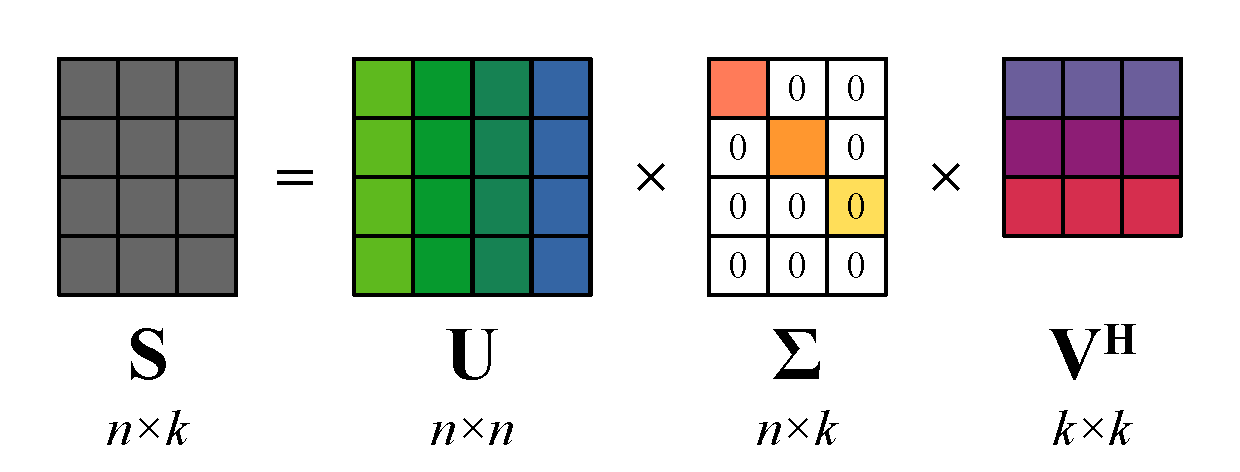
\includegraphics[width=\textwidth]{kep/reduced_svd_sajat_1.pdf}
                    \caption{Teljes SVD.}
                    \label{fig:reduced_svd_sajat_1}
                \end{subfigure}
                \begin{subfigure}{0.48\textwidth}
                    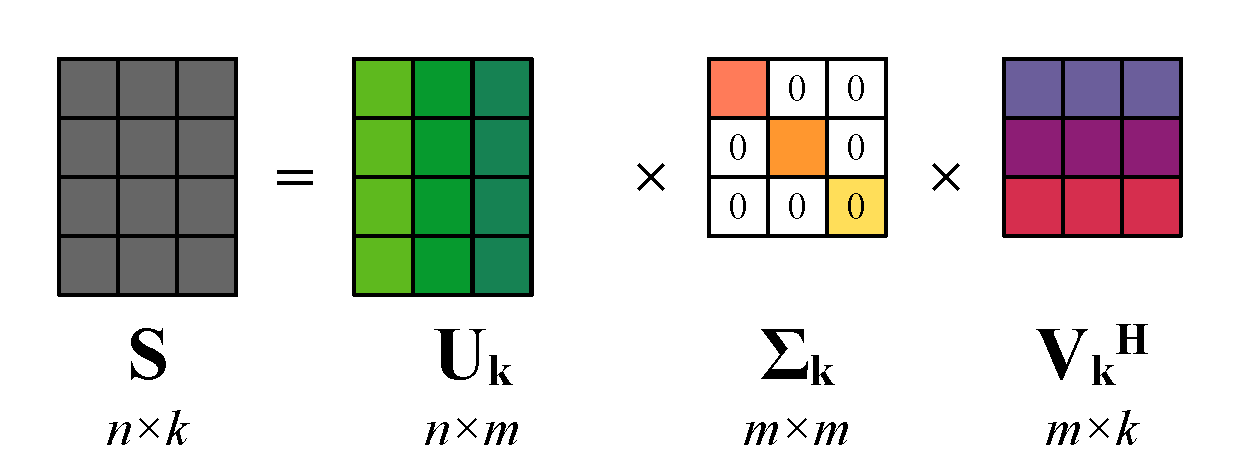
\includegraphics[width=\textwidth]{kep/reduced_svd_sajat_2.pdf}
                    \caption{Kompakt SVD.}
                    \label{fig:reduced_svd_sajat_2}
                \end{subfigure}
                \begin{subfigure}{0.48\textwidth}
                    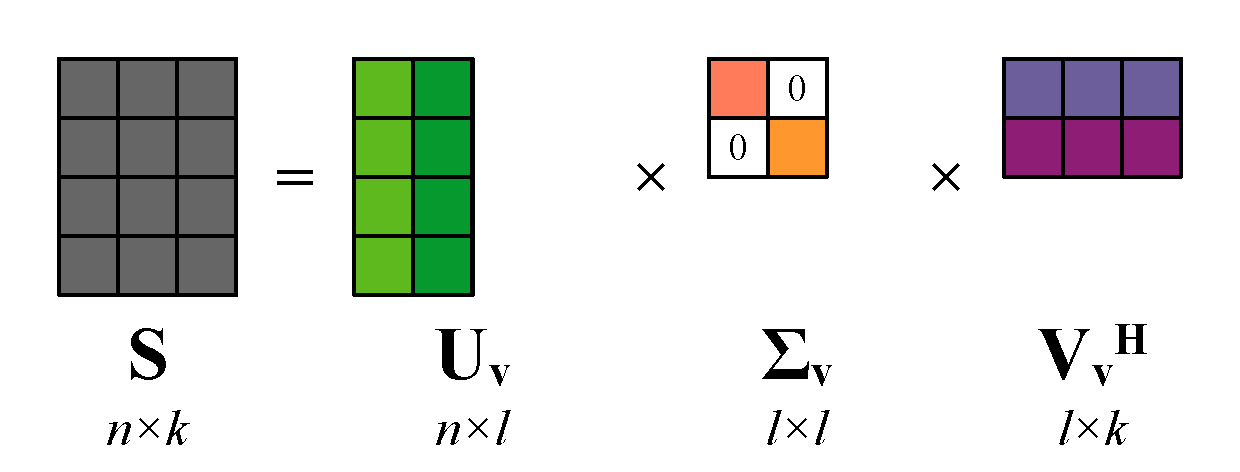
\includegraphics[width=\textwidth]{kep/reduced_svd_sajat_3.pdf}
                    \caption{Vékony SVD.}
                    \label{fig:reduced_svd_sajat_3}
                \end{subfigure}
                \begin{subfigure}{0.48\textwidth}
                    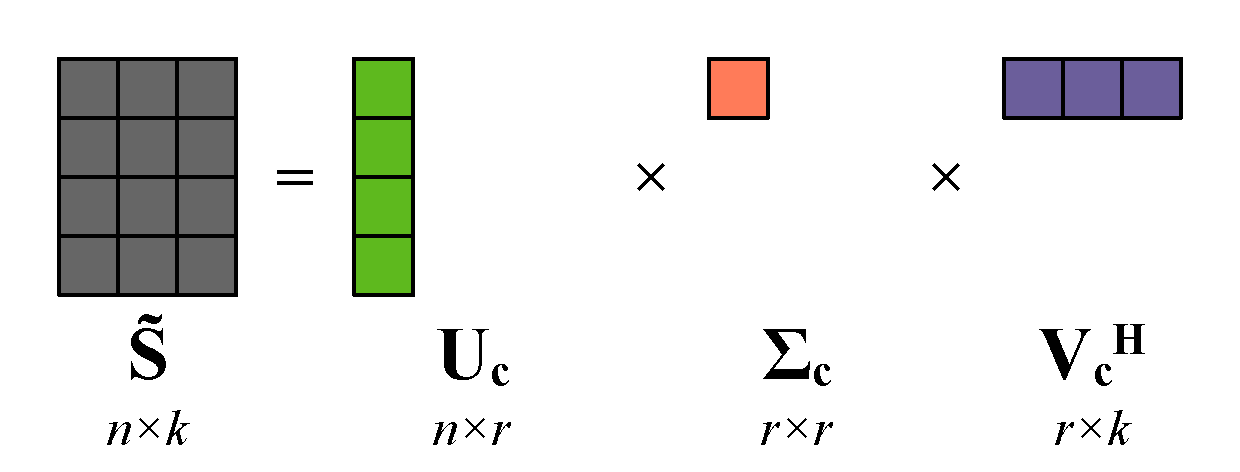
\includegraphics[width=\textwidth]{kep/reduced_svd_sajat_4.pdf}
                    \caption{Csonkított SVD.}
                    \label{fig:reduced_svd_sajat_4}
                \end{subfigure}
                \caption{Az SVD különböző változatai \cite{WikipediaSVD}.}
                \label{fig:reduced_svd_sajat}
            \end{figure}
            %TODO wikipedia szerint thin, compact és truncated. Lehet, hogy föntebb is át kéne írni, hogy hogy érdemes kiszámolni
            A takarékos SVD változatok \aref{fig:reduced_svd_sajat}. ábrán láthatóak olyan esetben, amikor $k < n$. Ezen belül a teljes SVD az, aminél ${\bf \Sigma}$ ugyanolyan méretű, mint a felbontott ${\bf S}$ mátrix, ezzel a változattal írtam fel előzőleg a mintamátrix felbontását (\ref{fig:reduced_svd_sajat_1}. ábra).
            \par
            A kompakt SVD a következőkben különbözik a teljes SVD-től. Éljünk a következő elnevezeéssel: $m=\min(n,k)$. Az ${\bf U}$ mátrixból kihagyjuk azokat az oszlopokat, amelyekhez nem tartozik sem szinguláris érték, sem ${\bf \adj{V}}$-beli oszlop, és hasonlóan ${\bf \adj{V}}$ soraival is, de az ${\bf U}$ és ${\bf \adj{V}}$ mátrixok közül egyszerre csak az egyiknek a megcsonkítására lehet szükség $n$ és $k$ viszonyától függően. Ezen kívül a ${\bf \Sigma}$ mátrixnak is kihagyjuk a csupa 0 részét, amely az utolsó $n-m$ sora vagy az utolsó $k-m$ oszlopa, így egy $m \times m$ méretű diagonálmátrix lesz belőle, aminek minden diagonáleleme egy szinguláris érték. Ekkor a kompakt SVD-ben ${\bf U_k} \in \mathbb{C}^{n\times m}, {\bf\Sigma_k} \in \mathbb{C}^{m\times m}, {\bf \adj{V_k}} \in \mathbb{C}^{m\times k}$. A kompakt SVD a teljes változathoz képest nem jár információveszteséggel ${\bf S}$-re nézve. Az SVD-nek ez a változata használható MATLAB-ban, ha megadjuk az \verb|svd()| függvénynek a \verb|`econ`| opciót.
            \par
            A vékony SVD egy következő redukcióval jön létre a kompakt változatból. A kompakt SVD esetén még a szinguláris értékek között lehetnek 0 értékűek, amelyek a ${\bf \Sigma_v}$ főátlójának utolsó elemei. Tegyük fel, hogy $l$ számú nemnulla szinguláris érték van. A 0 szinguláris értékekhez tartozó ${\bf U_v}$-beli oszlopok és ${\bf \adj{V_v}}$-beli sorok szintén nem hordoznak hasznos információt, így ezektől is meg lehet szabadulni, valamint ${\bf \Sigma_v}$-ből is elég csak azt az $l\times l$-es bal felső részmátrixot megtartani, aminek a főátlójában a nemnulla szinguláris értékek vannak. Ekkor ${\bf U_v} \in \mathbb{C}^{n\times l}, {\bf \Sigma_v} \in \mathbb{C}^{l\times l}, {\bf \adj{V_v}} \in \mathbb{C}^{l\times k}$. Mivel itt már azt vizsgáljuk, hogy a szinguláris értékek 0 értékűek-e, felmerül az árbázolási hiba kérdése, ami miatt tévesen sokkal több szinguláris értéket is pozitívnak vélhet az algoritmus, mint amennyi valójában jelentős méretű. Erre a problémára nyújt megoldást az ábrázolási hibahatár megadása. Még ez a változat sem jár információvesztéssel, de az ábrázolási hibahatár használata miatt más numerikus pontatlanságból adódó zaj fogja terhelni a vékony SVD felbontásból visszaállított ${\bf S}$ mátrixot, mint az előző két esetben.
            \par
            Végül pedig a csonkított változat olyan, hogy csak a legnagyobb $r$ számú szinguláris érték, valamint az ezekhez tartozó ${\bf U}$-beli oszlopok és ${\bf \adj{V}}$-beli sorok számolódnak ki. Az $r$ szám egy előre megadott konstans. Ekkor ${\bf U_c} \in \mathbb{C}^{n\times r}, {\bf \Sigma_c} \in \mathbb{C}^{r\times r}, {\bf \adj{V_c}} \in \mathbb{C}^{r\times k}$. Ebben az esetben már az ${\bf S}$ mátrixnak csak egy kisebb rangú reprezentációja, ${\bf \tilde{S}}$ állítható elő a ${\bf U_c \times\Sigma_c\times\adj{V_c}}$ szorzatként.
    \section{Példa szimuláció}
        A POD működésének demonstrálására a konzulensem, Dr. Bilicz Sándor segítségével írtam egy MATLAB szkriptet. A szkript egy egydimenziós véges differencia közelítést használó modell tranziens viselkedését szimulálja, pontosabban az elektromos és mágneses tér alakulását. A megoldást többféleképpen számítja ki, teljes és redukált bázisú változatban is, hogy ezek összehasonlíthatóak legyenek. Ez a szimuláció egy nagyon egyszerű problémán mutatja be a POD működését, ennél a konkrét feladatnál nincs jelentőssége a redukált bázisban való számításnak, mert a szimuláció anélkül is nagyon kevés erősorrást igényel. Azért célszerű egy egyszerű modellen bemutatni a módszert, mert a teljes rendű szimuláció is gond néklül lefuttatható, így a modellredukcióból adódó hibákat is vizsgálni lehet. A probléma egyszerűségét mutatja, hogy már 50 diszkretizáló ponttal is jól leírható a rendszer, ami nagyon kevés szabadsági foknak számít a gyakorlati jelentősségű szimulációkhoz viszonyítva.
        \subsection{A modell}
            A szimulációval egy kör keresztmetszetű, $a$ sugarú, végtelen hosszú, véges vezetőképességű vezetőben létrejövő mágneses és elektromos teret vizsgáltam. \Aref{fig:modell}. ábrán látható módon áll össze a modell. 
            \par
            \begin{figure}[h!]
                \centering
                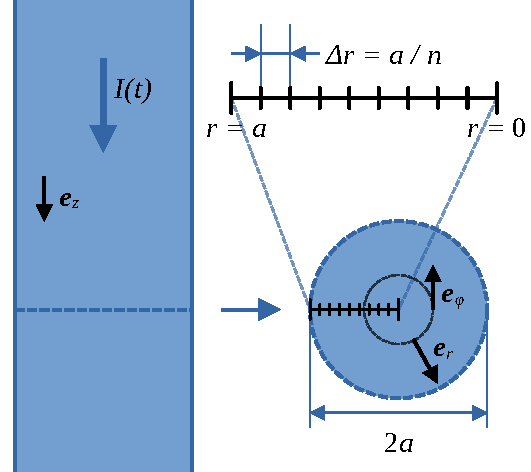
\includegraphics[width=0.48\textwidth]{kep/modell.pdf}
                \caption{A szimulált modell.}
                \label{fig:modell}
            \end{figure}
             A vezető rúd keresztmetszete a szaggatottal jelölt kör. A vezető hengernek $\sigma$ fajlagos vezetése és $\mu=\mu_0$ permeabilitása van. A használt henger-koordinátarendszer bázisvektorai ${\bf e}_{z}, {\bf e}_{\varphi}$ és ${\bf e}_{r}$. A vezető henger szimmetriatengelye $z$ irányú és szintén $z$ irányú benne a felületi áramsűrűség vektora is, ez az áramsűrűség a vezető hossza mentén nem változik. A modell általában $z$ irányú eltolásra és a szimmetriatengely körüli ($\varphi$ irányú) forgatásra invariáns, így  csak az egyes mennyiségek $r$ sugártól való függését kell vizsgálni, emiatt egydimenziós a modell.
             \par
             A vezető keresztmetszetére elő van írva az összesített áram időfüggvénye, $i(t)$, de a skin-hatás miatt a vezető belsejében nem egyenletes az áramsűrűség, hanem a sugár mentén haladva változik. Ugyanígy a vezető belsejében létrejövő $H_\varphi$ és $E_z$ is függ a sugártól. Ezek a mennyiségek továbbá időfüggőek is, de a vezető henger önindukciója miatt nem pontosan a gerjesztéssel együtt változnak. Ezeknek a mennyiségeknek az időbeli alakulása a kérdés, ezeket határozza meg a szimuláció egy adott gerjesztés mellett. A kísérleteim során az össz-áram időfüggvénye egy fél szinuszhullám, egyébként nulla.
            \par
            A modell például egy villámhárító földelő vezetőjében létrejövő elektromágneses tér alakulásának a vizsgálatára használható, amikor a villám meghatározza a villámhárítón folyó áramot.
        \subsection{Teljes rendű megoldás}
            A félév során készített szimuláció a következőképpen épül fel.
            \par
            A rendszer 0 kezdeti állapotból indul, tehát kezdetben a hengerben nem folyik áram és emiatt 0 benne a mágneses és elektromos térerősség is. Az eredő $i(t)$ a felszíni mágneses térerősségen keresztül van előírva.
            \begin{equation}
                H_{\varphi}(r=a,t) = \dfrac{i(t)}{2\pi a}
            \end{equation}
            \par
            Kétféle időlépéses módon készül megoldás a problémára, az egyik egy egyszerű előrelépő Euler sémát használ, a másik pedig a MATLAB beépített \verb|ode45()| függvényét, ami Runge-Kutta sémára épül és adaptív az időlépése. Mindkét megoldástípushoz szükség van arra, hogy a rendszer adott pillanatbeli állapotából, amit $H_{\varphi}(r,t)$ teljesen leír, ki lehessen számítani $H_{\varphi}$ idő szerinti parciális deriváltját. Ennek a parciális deriváltnak a segítségével aztán lehet előre léptetni az időlépéses sémákat, amiből egy $\Delta t$ idővel későbbi $H_{\varphi}(r,t+\Delta t)$ állapot adódik.
            \begin{align}
                \label{equ:fe}
                H_{\varphi}(r,t+\Delta t) \approx & \dfrac{\partial H_{\varphi}(r,t)}{\partial t} \cdot \Delta t
            \end{align}
            Az előrelépő Euler séma időléptetése \aref{equ:fe}. egyenletben látható. Ez az időlépéses séma könnyen használhatatlan lesz, ha rosszul választjuk meg a térbeli diszkretizáló távolságot, ($\Delta r$), valamint az időlépés hosszát ($\Delta t$). A szimuláció előtt a szkript konvergenciavizsgálatot végez, amihez a következő képletet használja:
            \begin{align}
                F &= \dfrac{\alpha \Delta t}{\Delta r^2}, \quad \alpha = \dfrac{1}{\mu \sigma}
            \end{align}
            A megoldás csak akkor konvergens, vagyis használható, ha $F<0.5$. Ez az $F$-re vonatkozó határ Descartes-koordináták esetére van levezetve, de a tapasztalatunk szerint hengerkoordináták esetében is helytálló.
            \par
            A Maxwell-egyenleteknek a modellben használt alakja \aref{equ:maxwell}. egyenletrendszerben látható. Magneto-kvázistacionárius közelítést használok, valamint a $\sigma$ és $\mu$ anyagjellemzők egy-egy időben állandó skalárral leírhatóak.
            \begin{equation}\label{equ:maxwell}
                \begin{aligned}
                \rot \textbf{H}~&=~{\bf J} \\
                \rot \textbf{E}~&=~-\dfrac{\partial \textbf{B}}{\partial t} \\
                \divergence \textbf{B}~&=~0 \\
                \divergence \textbf{E}~&=~0 \\
                \textbf{B}~&=~\mu \textbf{H} \\
                \textbf{J}~&=~\sigma\textbf{E}
                \end{aligned}
            \end{equation}
            A gerjesztő áram csak $z$ irányú, így az Amp\`ere-törvény miatt a rá merőleges $\textbf{H}$ mágneses térerősségnek csak $\varphi$ irányú komponense lesz. A $\textbf{H}$ változása pedig a Faraday-törvény miatt szintén csak $z$ irányú, $\sigma\textbf{E}$ vezetési áramot hozhat létre, tehát az eredő $\textbf{J}$ áramnak mindig csak $z$ irányú komponense lesz, a $\textbf{H}$ térerősségnek pedig csak $\varphi$ irányú komponense. Így elég csupán ezekkel a komponensekkel foglalkozni, amelyeket mint skalármennyiségekként lehet meghatározni.
            \begin{equation}\label{equ:komponens}
                \begin{aligned}
                    \textbf{H} &= H_{\varphi}\textbf{e}_\varphi\\
                    \textbf{J} &= J_{z}\textbf{e}_z\\
                    \textbf{E} &= E_{z}\textbf{e}_z
                \end{aligned}
            \end{equation}
            \par
            \Aref{equ:maxwell}. egyenletrendszer kifejezéseit átrendezve \aref{equ:dhdt}. egyenletben látható összefüggéshez jutunk. Ennek egy véges differenciálokkal kifejezett alakját használva áll elő a szimuláció során az idő szerinti derivált közelítő értéke.
            \begin{equation}\label{equ:dhdt}
                \begin{aligned}
                    \dfrac{\partial \textbf{H}}{\partial t} &= -\dfrac{1}{\sigma\mu}\rot\rot\textbf{H}\\%TODO véges differenciás képlet ehhez
                \end{aligned}
            \end{equation}
            \par
            Mivel a hengerre az összáram időfüggvénye adott, így ezzel együtt a felszíni mágneses térerősség is adott. Ezen kívül a forgási szimmetria miatt az $r=0$ pontban is ismerten $\textbf{H}_{\varphi}=0$ a gerjesztéstől függetlenül. Ha $n$ számú diszkretizáló ponttal dolgozunk, akkor tehát két pontra már adott a megoldás $\textbf{H}_{\varphi}$-re vonatkozóan, így $n-2$ pontra kell azt kiszámítani. \Aref{equ:DhDt}. egyenlet szerint véges differencia közelítéssel kiszámítható egy adott időlépésbeli mágneses térerősség eloszlásából annak az idő szerinti deriváltja, ami felhasználható az időléptetéshez mindkétféle időlépéses sémában:
            \begin{equation}\label{equ:DhDt}
                \begin{aligned}
                    \dfrac{\Delta \textbf{H}}{\Delta t} &\approx -\dfrac{1}{\sigma\mu}\mathbf{R}\textbf{H}
                \end{aligned}
            \end{equation}
            ahol $\mathbf{R}$ a $\rot\rot$ operátor véges differencia közelítésének mátrixa.
            Így az időléptetéshez nincs szükség az $\textbf{E}$ vagy $\textbf{J}$ terek kiszámolására, ezek meghatározása csak egy utófeldolgozási lépést jelent.
        \subsection{Redukált rendű megoldás}
            A teljes rendű megoldás időben a gerjesztő impulzus hosszának kétszereséig terjed a kísérleteimben ($T$ a teljes időtartam hossza). Ennyi idő elteltével már a tranziens válasz lényegi része lejátszódik a tapasztalataim szerint. Ennek az időtartamnak az első kis részére, $cT$ időtartamra keletkező megoldás szolgál a POD bemeneti mintamátrixaként, amiben egy-egy oszlop, vagyis minta, egy adott $t$-hez tartozó időlépésre érvényes megoldás $H_{\varphi}$-re, amit $\textbf{H}_{\varphi}(t)$-vel jelölök. A kísérleteim során $c=\num{0,07}$, $\num{0,15}$ és $\num{0,3}$ értékeket próbáltam ki.
            \begin{equation}\label{equ:minta}
                \begin{aligned}
                    \textbf{S} &= \begin{bmatrix}
                        \textbf{H}_{\varphi}(0\cdot\Delta t)\quad
                        \textbf{H}_{\varphi}(1\cdot\Delta t)\quad
                        \textbf{H}_{\varphi}(2\cdot\Delta t)\quad
                        \hdots\quad
                        \textbf{H}_{\varphi}(k\cdot\Delta t) \end{bmatrix}
                \end{aligned}
            \end{equation}
            \par
            Megjegyzem, hogy valószínűleg nem mindig célszerű a mintavételezett időtartam összes időlépését felhasználni $\textbf{S}$ megkonstruálásához. Ha jól meg tudjuk választani a mintákat, akkor valószínűleg elég a redukált bázis számosságánál csak legfeljebb \qtyrange{1}{2}{} nagyságrenddel nagyobb számú minta a rendszerből, attól függetlenül, hogy hány időlépést tartalmazó időintervallumot mintavételezünk. Ennek a csökkentett mintavételezésnek a hatását a félév során már nem volt időm megvizsgálni.
            \par
            A $\Psi$ bázist a MATLAB \verb|svd()| függvényével állítom elő. Ez a függvény mint egy melléktermékként az $\textbf{S}$ mátrix teljes SVD felbontását kiszámítja, így a szinguláris értékek mátrixát, $\mathbf{\Sigma}$-t is. A szinguláris értékek egy futtatásból \aref{fig:sigma}. ábrán láthatóak. Az ábrán elég szembetűnő, hogy a szomszédos szinguláris értékek között elég nagy különbség van, főként az első néhány szinguláris értéknél. Ez a redukált rendű szimuláció szempontjából egy nagyon jó hír, hiszen ekkor ha csak az első néhány bázisvektort használjuk is, a megoldás jól fogja közelíteni a teljes rendűt.
            \begin{figure}[h!]
                \centering
                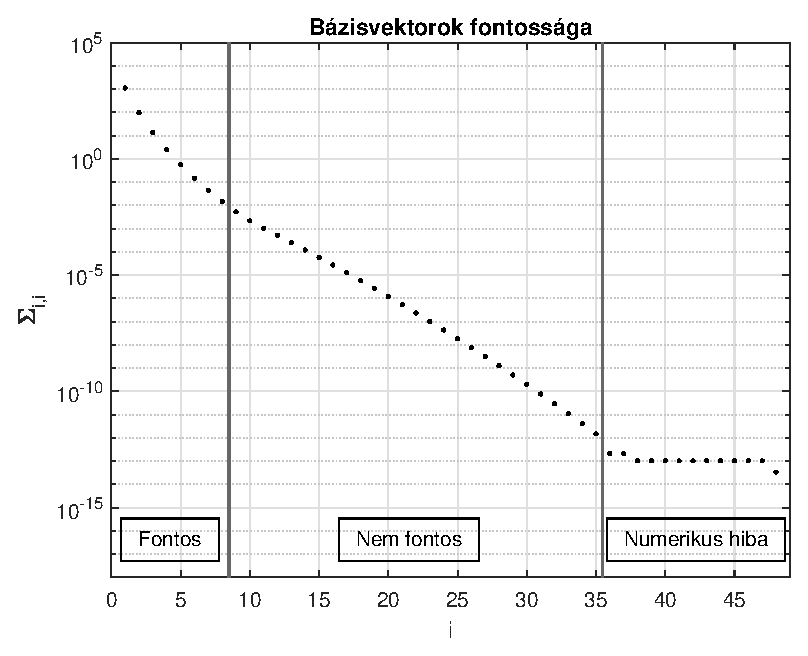
\includegraphics[width=0.6\textwidth]{kep/euler_0.15_4_sv.eps}
                \caption{A szinguláris értékek az előrelépő Euler megoldásból.}
                \label{fig:sigma}
            \end{figure}
            \Aref{fig:sigma}. ábrán bejelölt határvonalak közül a ,,numerikus hibá''-t elválasztó vonal elég egyértelmű helyen van, ott van egy törés az értékek sorozatában. Ezzel szemben a ,,fontos'' és ,,nem fontos'' részek közötti vonal pontos helye már nem magától értetődő, attól függ, hogy mekkora hibát engedhetünk meg a szimuláció során.
            \par
            A numerikus hibák által dominált szinguláris értékek egymástól csak nagyon kevéssé térnek el, a többség majdnem pontosan \num{1e-13} értékű. A legnagyobb szinguláris érték pedig \num{1e3} körüli. Ezek hányadosa tehát körülbelül \num{1e16}. A számok MATLAB-ban a sztenderd double formátumban tárolódnak el, amiknek az értékes helyiértékeket tároló része, vagyis a mantissza effektíve 53 bites. Az 53 biten ábrázolható legnagyobb szám ($2^{53}-1$) körülbelül \num{9,0072e15}, ami jól illeszkedik a tapasztalt relatív pontossághoz. Gyakorlatilag amikor két double-ként tárolt számot adna össze a számítógép, amelyek hányadosa eléri a $2^{53}$-t, akkor az exponensek egyeztetéséhez a kisebb szám mantisszáját legalább 53 helyiértékkel kell léptetelni, de ezáltal az összes értékes bit kiléptetődik és 0-kkal töltődik fel a helyük. Emiatt az összeadás eredménye pontosan a nagyobb szám lesz, mintha hozzá sem adtuk volna a kisebbet, így a kisebb szám effektíve 0. Az SVD kiszámolása közben  ilyen double összeadások miatt lehetetlenül el a legnagyobbhoz képest nagyon kis szinguláris értékek és az ezekhez tartozó szinguláris vektorok kiszámolása.
            \par
            Az SVD kimenetei között van az $\textbf{U}$ mátrix is, ami az új bázisvektorokat ($\textbf{u}_i$) tartalmazza fontosság szerint csökkenő sorrendben az oszlopaiban. Ezek közül a legfontosabb $r$ db-ot megtartva és azonos sorrendben egy új mátrixba rendezve kapjuk a redukált bázis $\mathbf{\hat{U}}$ mátrixát, ami az új, redukált bázisból a standard bázisba való áttérés mátrixa.
            \begin{equation}\label{equ:uhat}
                \begin{aligned}
                    \mathbf{\hat{U}} =
                    \begin{bmatrix}
                        \textbf{u}_1\quad\textbf{u}_2\quad\textbf{u}_3\quad\hdots\quad\textbf{u}_r
                    \end{bmatrix}
                \end{aligned}
            \end{equation}
            \par
            Érdemes szemügyre venni magukat a bázisvektorokat is, amelyek közül néhány \aref{fig:bazis}. ábrán látható. Fontos megjegyezni, hogy az egyes bázisvektorok valódi térerősség-eloszlásokat jelentenek, amelyeknek valamilyen lineáris kombinációjával írjuk le a rendszer aktuális állapotát.
            \begin{figure}[h]
                \centering
                \begin{subfigure}{0.48\textwidth}
                    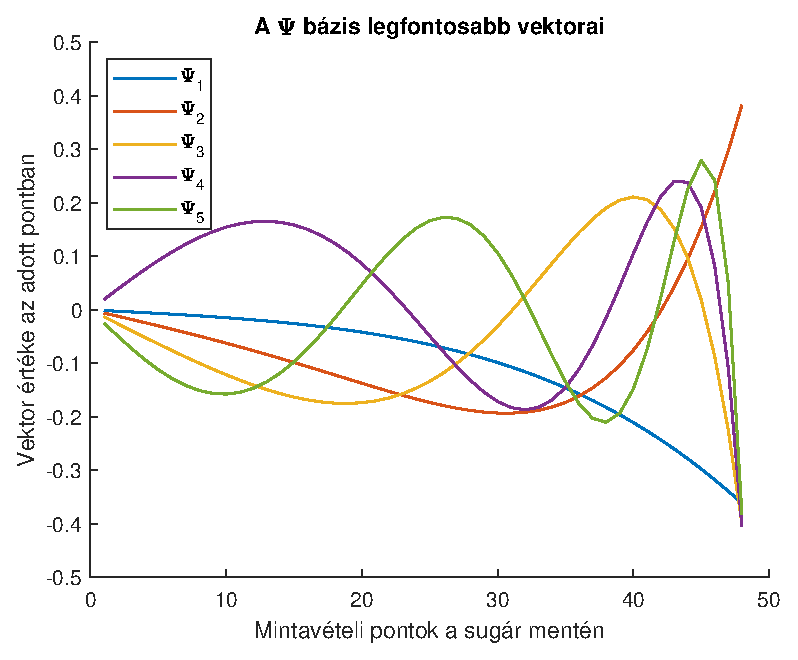
\includegraphics[width=\textwidth]{kep/euler_0.15_4_base_1_5.eps}
                    \caption{Az öt leglényegesebb vektor.}
                \end{subfigure}
                \begin{subfigure}{0.48\textwidth}
                    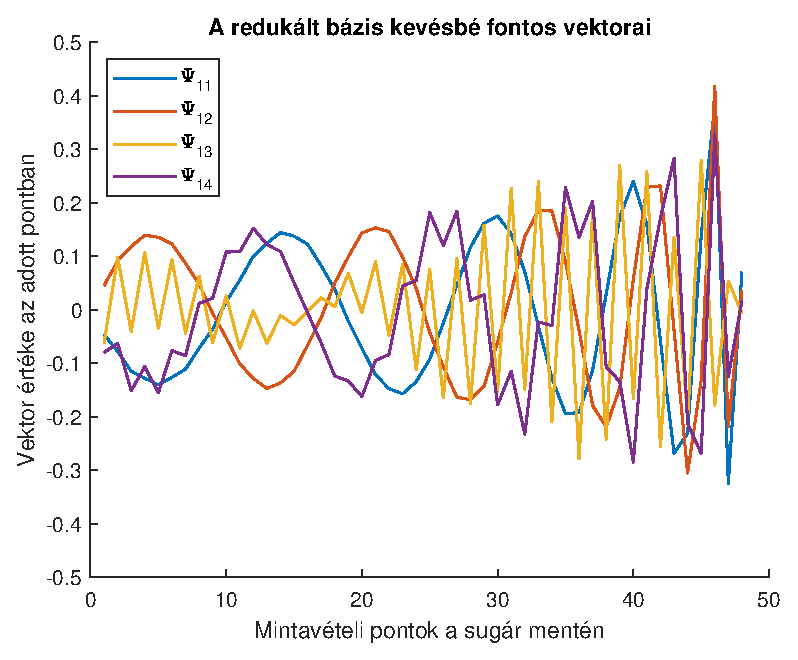
\includegraphics[width=\textwidth]{kep/euler_0.15_4_base_11_14.eps}
                    \caption{Négy lényegtelen vektor.}
                \end{subfigure}
                \caption{A $\Psi$ bázis néhány vektora.}
                \label{fig:bazis}
            \end{figure}
            \par
            Mivel ${\bf U} \in \mathbb{C}^{n \times n}$ unitér, ezért:
            \begin{equation}
                \begin{aligned}
                    \mathbf{U}\adj{\mathbf{U}} = \adj{\mathbf{U}}\mathbf{U} = \mathbf{I}_{n\times n}
                \end{aligned}
            \end{equation}
            De a csonkítás miatt az $\mathbf{\hat{U}} \in \mathbb{C}^{n \times r}$ mátrixra már csak a következő igaz:
            \begin{equation}
                \begin{aligned}
                    \adj{\mathbf{\hat{U}}}\mathbf{\hat{U}} = \mathbf{I}_{r\times r}
                \end{aligned}
            \end{equation}
            Az $\mathbf{\hat{U}}$ mátrixnak egy további fontos tulajdonsága, hogy ennek a mátrixnak a segítségével lehet egy standard bázisban felírt $\mathbf{x} \in \mathbb{C}^{n}$ vektort a redukált $\Psi'$ bázisba vetíteni, valamint a fordított irányú bázistranszformációt is el lehet végezni $\adj{\mathbf{\hat{U}}}$ segítségével:
            \begin{equation}
                \begin{aligned}
                    \adj{\mathbf{\hat{U}}}\mathbf{x} &= \mathbf{y}\\
                    \mathbf{\hat{U}}\mathbf{y} &= \mathbf{x'} \approx \mathbf{x}
                \end{aligned}
            \end{equation}
            ahol $\mathbf{y} \in \mathbb{C}^{r}$ a $\Psi'$ bázisbeli reprezentációja $\mathbf{x}$-nek. Az iylen irányú éttérés információvesztéssel jár, de a POD tulajdonságai miatt az euklideszi távolság $\mathbf{x}$ és $\mathbf{x'}$ között kicsi olyan $\mathbf{x}$-ekre, amelyek előfordulhatnak a rendszer állapotai között.
            \par
            Az időléptetéshez még szükséges az $\mathbf{R}$ mátrixnak a vetítése a $\Psi'$ bázisba, vagyis $\mathbf{R}_{\Psi}$ kiszámolása. Ezt a jól ismert bázistranszformációs képlet alapján lehet megtenni:
            \begin{equation}
                \adj{\mathbf{\hat{U}}}\mathbf{R}\mathbf{\hat{U}} = \mathbf{R}_{\Psi}
            \end{equation}
            Az eddigiek felhasználásával pedig kiszámíthatjuk az $\mathbf{R}\mathbf{x'}$ egy közelítését a $\Psi'$ bázisban anélkül, hogy az egyes időlépések közben bármikor is vissza kellene térni a standard bázisba:
            \begin{equation}
                \mathbf{R}_{\Psi}\mathbf{y} =
                \adj{\mathbf{\hat{U}}}\mathbf{R}\mathbf{\hat{U}}\mathbf{y} =
                \adj{\mathbf{\hat{U}}}\mathbf{R}\mathbf{x'}
            \end{equation}
            \par
            A redukált bázisban való számolás összefoglalva a következőképpen zajlik. A mintavételezett időintervallum alapján megkonstruálom a $\Psi'$ bázist. Ebbe a bázisba vetítem a mintavételezés végén a rendszer aktuális állapotát, valamint a $\rot\rot$ operátor mátrixát. Ezek után már csak a redukált bázisban számolok tovább. A szimuláció végén a megoldást visszavetítem a standard bázisba, de ezt a vetítést nem feltétlenül kell megtenni minden időlépés minden térbeli pontjára, mind térben, mind időben lehet szelektálni.
    \section{Eredmények}
        Olyan alkalmazások esetén, amikor a tranziens szimulációnál lényeges erőforráscsökkenéssel jár a POD alkalmazása, nem érdemes a teljes rendű szimulációt végig futtatni, csak a POD bemenetének használt időtartam végéig, legfeljebb kicsivel tovább az esetleges nyilvánvaló hibák felismerése céljából. A vizsgálódásomhoz a teljes rendű szimulációt is végig futtattam, hogy össze lehessen hasonlítani a redukált megoldással. A teljes rendű Euler-séma megoldásának vízesésdiagramjai \aref{fig:vizeses}. ábrán láthatóak.
        \begin{figure}[h]
            \centering
            \begin{subfigure}{0.48\textwidth}
                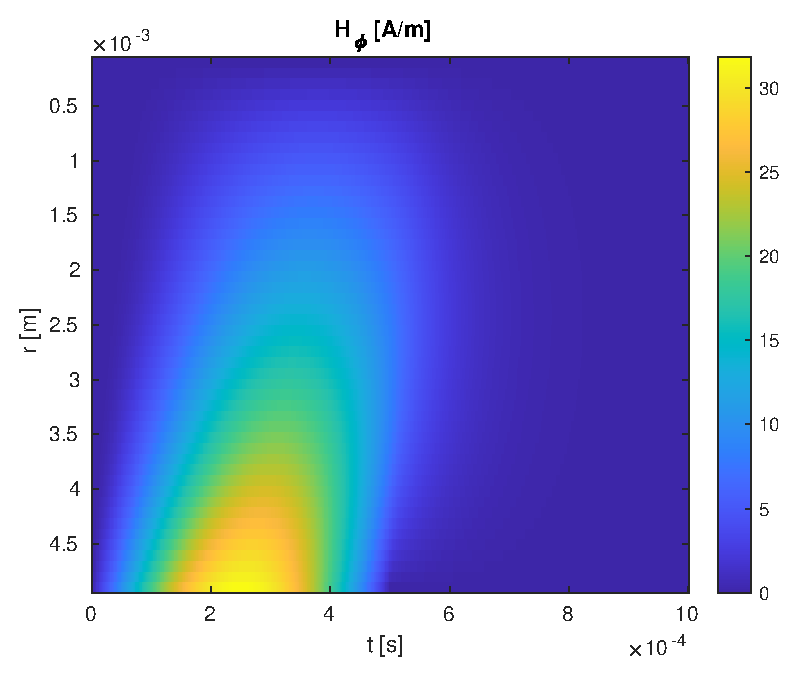
\includegraphics[width=\textwidth]{kep/euler_0.15_4_hphi_waterfall.eps}
                %\caption{$H_{\varphi}$ vízesésdiagramja}
            \end{subfigure}
            \begin{subfigure}{0.48\textwidth}
                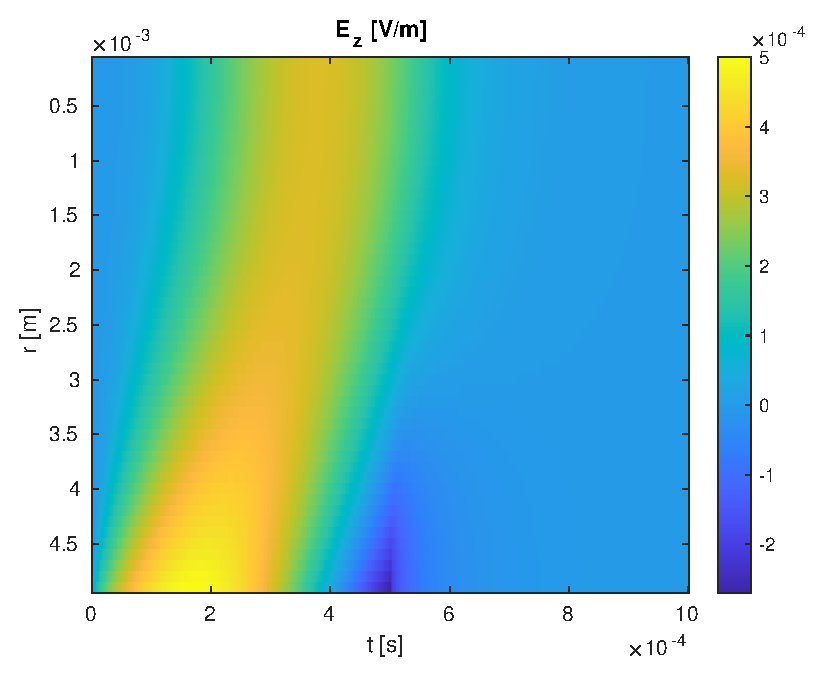
\includegraphics[width=\textwidth]{kep/euler_0.15_4_ez_waterfall.eps}
                %\caption{$E_{z}$ vízesésdiagramja}
            \end{subfigure}
            \caption{Teljes rendű megoldások az előrelépő Euler sémával.}
            \label{fig:vizeses}
        \end{figure}
        \par
        Külön megoldást készítettem azonos paraméterekkel, mind az egyszerű előrelépő Euler, mind a Runge-Kutta sémák használatával. Ezeknek az eredményei \aref{fig:sema}. ábrán láthatóak. Az ábrák alapján mindkét séma hasonlóan jó megoldást ad, így többnyire bármelyik használható. A továbbiakban elsősorban az Euler-sémán mutatom be a felmerülő jelenségeket.
        \begin{figure}[h]
            \centering
            \begin{subfigure}{0.48\textwidth}
                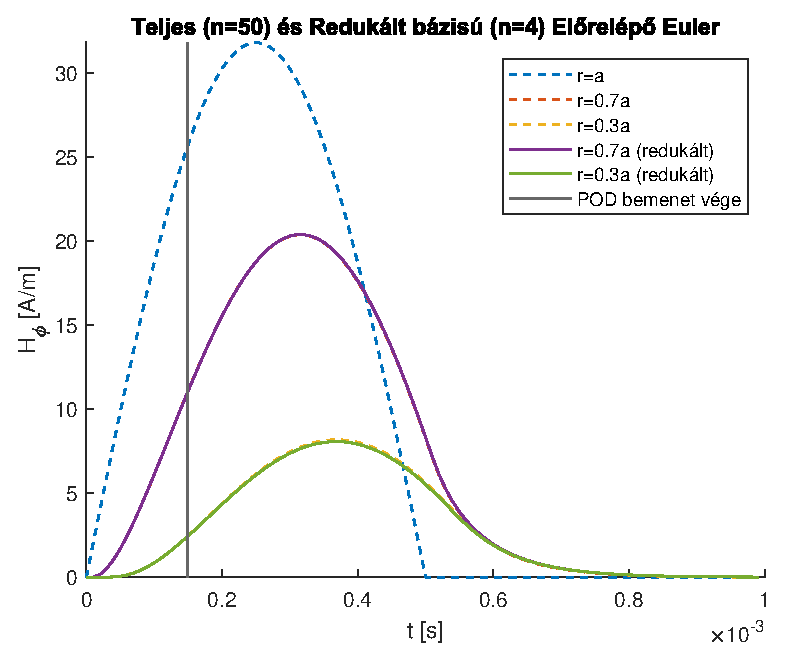
\includegraphics[width=\textwidth]{kep/euler_0.15_4_td.eps}
                \caption{Előrelépő Euler}
            \end{subfigure}
            \begin{subfigure}{0.48\textwidth}
                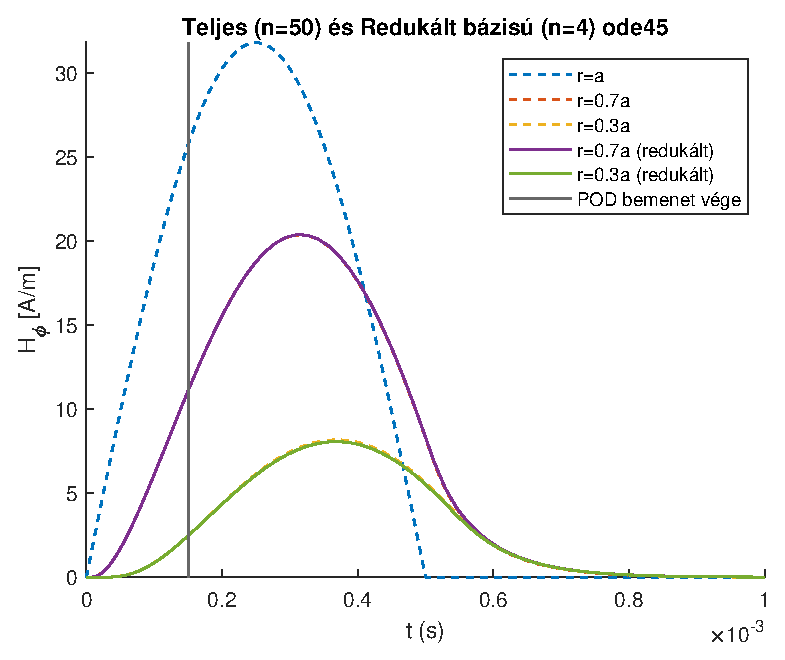
\includegraphics[width=\textwidth]{kep/ode45_0.15_4_td.eps}
                \caption{Runge-Kutta}
            \end{subfigure}
            \caption{Megoldások kétféle sémával, teljes és redukált bázisokban ($r=4$ és $c=0.15$).}
            \label{fig:sema}
        \end{figure}
        \par
        Amint az ábrán is látszik, azonos paraméterek mellett mindkét időlépéses séma esetén hasonlóan kis hibával működik a redukált rendű közelítés. Jobb kvantitatív képet kapunk a redukált bázisú szimuláció pontosságáról, ha a teljes rendű szimuláció összetartozó pontjához viszonyított relatív hibát, valamint az abszolút hibát vizsgáljuk. Ezek az eredmények \aref{fig:hiba}. ábrán láthatóak.
        \begin{figure}[h]
            \centering
            \begin{subfigure}{0.48\textwidth}
                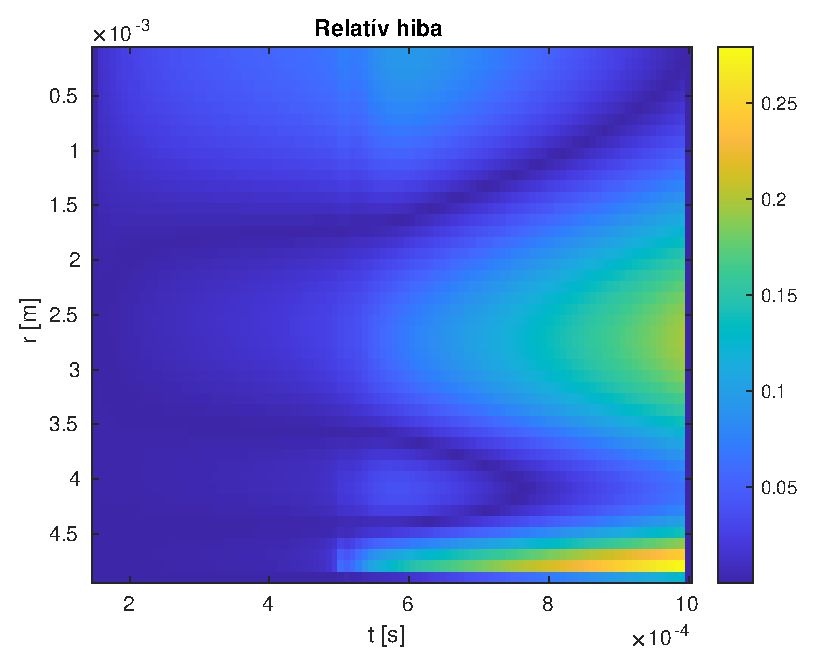
\includegraphics[width=\textwidth]{kep/euler_0.15_4_rel_error.eps}
                \caption{Hiba az összetartozó ponthoz képest.}
            \end{subfigure}
            \begin{subfigure}{0.48\textwidth}
                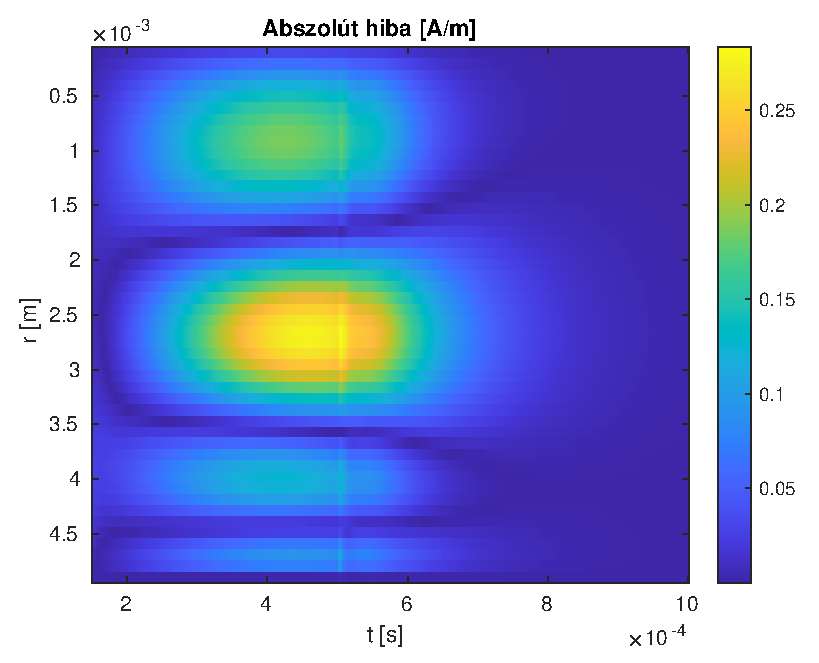
\includegraphics[width=\textwidth]{kep/euler_0.15_4_abs_error.eps}
                \caption{Abszolút hiba.}
            \end{subfigure}
            \caption{Az Euler séma abszolút és relatív hibája ($r=4$ és $c=0.15$).}
            \label{fig:hiba}
        \end{figure}
        A redukált rendű szimulációnak több paraméterét lehet szabadon megadni, ezek között valamilyen kompromisszumot kell találni. A kompromisszummal a cél, hogy még elfogadható hiba mellett, minél kisebb legyen az erőforrásigénye a redukált rendű közelítésnek. A megválasztható paraméterek a redukált bázis rendje, $r$, valamint a szimuláció teljes rendű részének hossza az teljes szimulált időtartamhoz képest, $c$. Tapasztalataim szerint a rögzített $c=0.15$ választás mellett $r=4$ az alsó határ, aminél még ránézésre használható közelítő eredmény adódik. Ha ugyanilyen $r=4$ mellett $c=0.07$-ot választottam, jelentősen megnőtt a közelítő megoldás hibája. Ez a megnövekedett hibájú megoldás \aref{subfig:keves_ido_rossz}. ábrán látható. Ebben a helyzetben az egyik megoldás, hogy a lecsökkentett $c$ mellé megnöveljük $r$-t, hogy a kevés és kevésbé reprezentatív mintahalmaz alapján is olyan bázist tudjon produkálni a POD, amiben jól leírható a rendszer. Enek a megoldásnak a hatása, pontosabban az $r=8$ választás hatása, \aref{subfig:keves_ido_jo}. ábrán látható.
        \begin{figure}[h]
            \centering
            \begin{subfigure}{0.48\textwidth}
                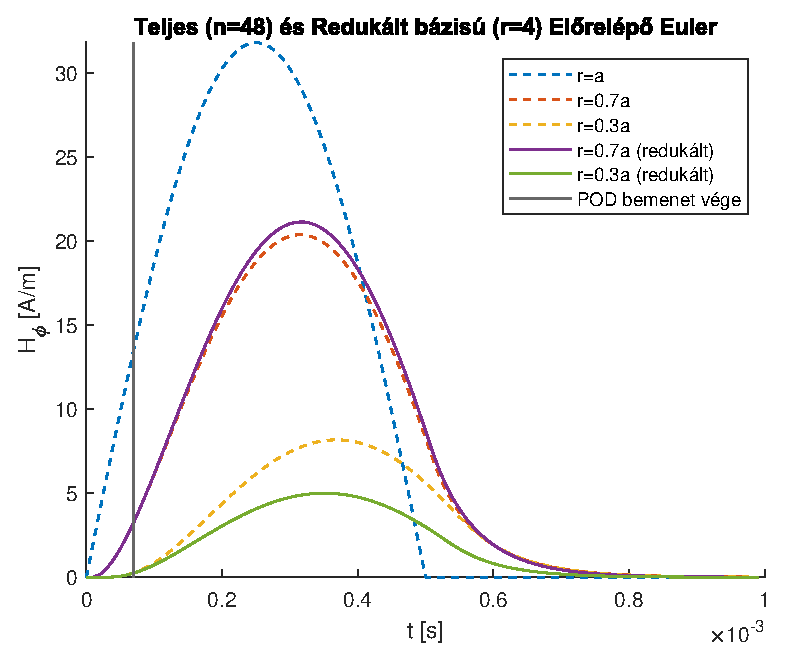
\includegraphics[width=\textwidth]{kep/euler_0.07_4_td.eps}
                \caption{Probléma}
                \label{subfig:keves_ido_rossz}
            \end{subfigure}
            \begin{subfigure}{0.48\textwidth}
                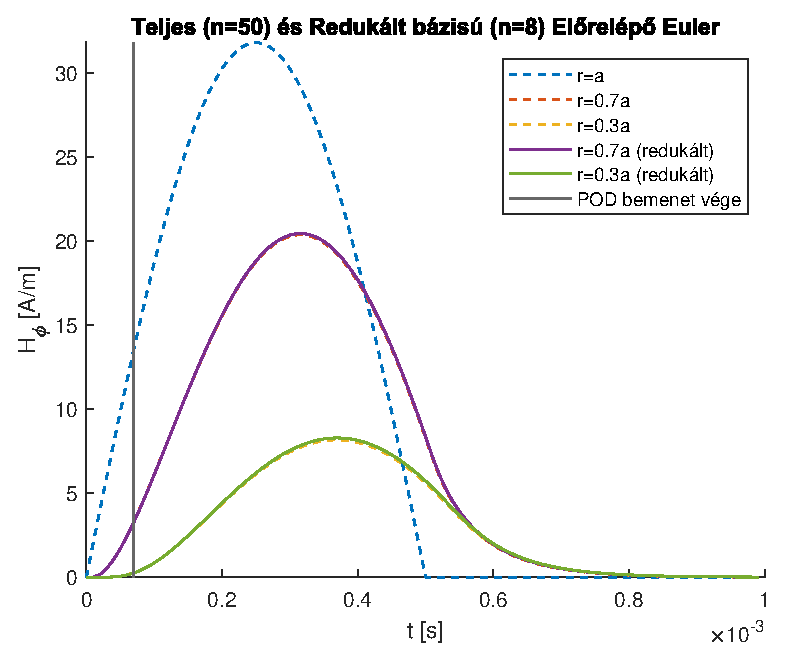
\includegraphics[width=\textwidth]{kep/euler_0.07_8_td.eps}
                \caption{Megoldás ($r=4 \rightarrow 8$)}
                \label{subfig:keves_ido_jo}
            \end{subfigure}
            \caption{Túl rövid a teljes rendű szimuláció időtartama ($c$).}
            \label{fig:keves_ido}
        \end{figure}
        \par
        Nagy hiba esetén a másik irányú korrekcióval is próbálkozhatunk, név szerint $c$ növelésével. Ennek a bemutatásához az eredeti $c=0.15$, $r=4$ paraméterektől az $r=2$ választással tértem el, ami már egy extrém kicsi szám erre a paraméterre, így nem várhatunk sok jót ettől a közelítő megoldástól. Az ehhez tartozó eredmények \aref{subfig:keves_vektor_rossz}. ábrán láthatóak. Ezek után a $c=0.3$ választással éltem, ennek az eredménye \aref{subfig:keves_vektor_jo}. ábrán látható. Megfigyelhető, hogy a teljes rendű megoldáshoz viszonyított hibával jelentős javulást nem értem el. A $c=0.3$ már azt jelenti, hogy a teljes időtartamnak egy számottevő részét a teljes rendű szimulációval számolom ki, ezek után már megkérdőjelezhető a POD használata a fennmaradó irőre. A redukált bázis kiszámolásának, valamint az ebben kiszámolt megoldás visszaalakításának többletmunkájától eltekintve még szélsőséges esetben is csak körülbelül $0.3$-szorosára csökkenthető az erőforrásigény az egész időtartamra végzett teljes rendű számításhoz képest. Ezek alapján ki lehet jelenteni, hogy a vizsgált rendszer elfogadható modellezésére nem elegendő 2 bázisvektor. A bázisvektorok számára vonatkozó határ mellett feltétlenül létezik a minták számára, valamint azok reprezentativitására vonatkozó határ is. Ez pedig azt korlátozza, hogy a teljes időtartamnak mennyire kis részére lehet korlátozni a mintavételezést. Természetesen ez a két határ különböző modelleknél más és más. 
        \begin{figure}[h]
            \centering
            \begin{subfigure}{0.48\textwidth}
                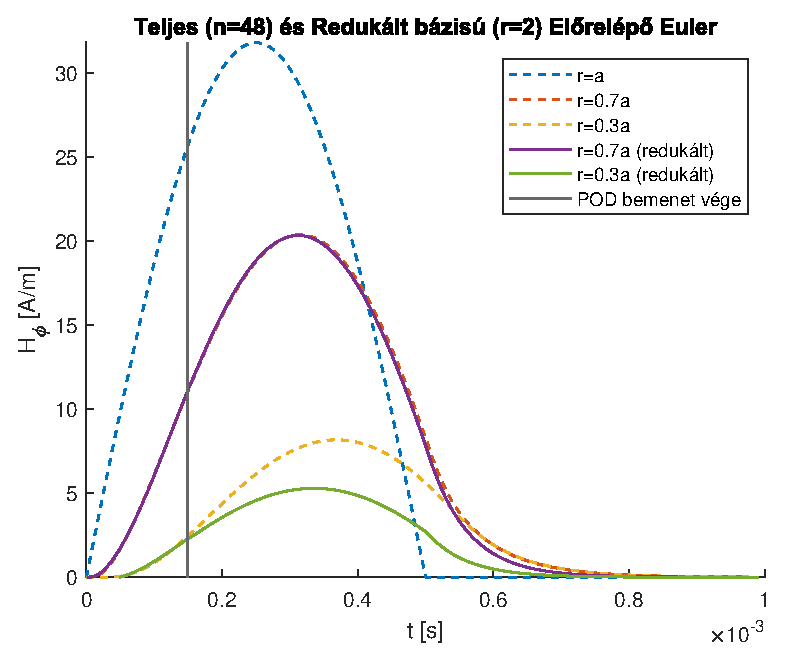
\includegraphics[width=\textwidth]{kep/euler_0.15_2_td.eps}
                \caption{Probléma}
                \label{subfig:keves_vektor_rossz}
            \end{subfigure}
            \begin{subfigure}{0.48\textwidth}
                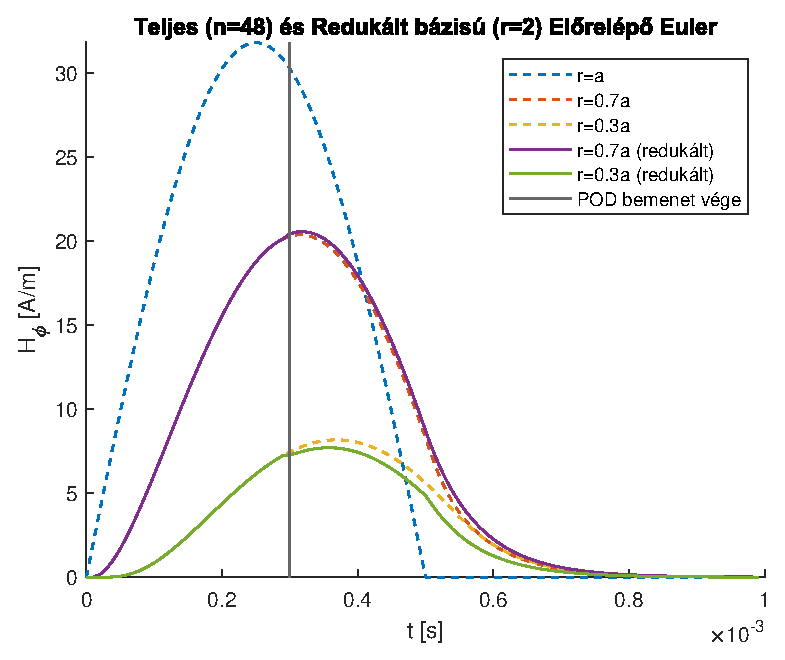
\includegraphics[width=\textwidth]{kep/euler_0.3_2_td.eps}
                \caption{Részleges megoldás ($c=0.15 \rightarrow 0.3$)}
                \label{subfig:keves_vektor_jo}
            \end{subfigure}
            \caption{Túl kicsi a bázisvektorok száma ($r$).}
            \label{fig:keves_vektor}
        \end{figure}
    \section{Összegzés}
        A félévben megismerkedtem a Proper Orthogonal Decomposition módszerrel és sikeresen alkalmaztam egy MATLAB-ban megírt FDTD alapú tranziens szimuláción. Megvizsgáltam a módszer néhány alapvető korlátját és jellegzetességét.
        \par
        A későbbiekben a POD potenciális alkalmazási területeit tervezem részletesebben felkutatni és az ígéretesebb alkalmazásoknál megvizsgálni, hogy van-e haszna a POD-nak az adott problémában. Ezek után pedig egy kiválasztott bonyolultabb problémára tervezem alkalmazni a módszert és elemezni a hatásait. Egy további kérdés lehet a redukált bázis használatából adódó hibák nagyságának és jellegének becslése a redukált rendű szimuláció futtatása előtt. Egy másik fennmaradó kérdés pedig az, hogy a mintamátrixba kerülő mintavektorokat hogyan érdemes kiválasztani a rendelkezésre álló adatok közül, és érdemes-e egyáltalán megszűrni az összes rendelkezésre álló adatot.
        \subsection*{Köszönetnyilvánítás}
            Köszönettel tartozom a konzulensemnek, Dr. Bilicz Sándornak a segítségért, ötletekért és iránymutatásért, amivel a munkám során támogatott.
    \bibliography{mybib}
    \bibliographystyle{plain}
\end{document}

%\cite{Henneron14}

%            \begin{figure}
%                \centering
%                \includegraphics[width=0.8\textwidth]{kep/szerkesztett/wstk-mighty-gecko-nagy.jpg}
%                \caption{WSTK + radio board.}
%                \label{fig:wstkmighty}
%            \end{figure}
% \cite{Anritsu}
%            \begin{figure}
%                \centering
%                \begin{subfigure}{0.48\textwidth}
%                    \includegraphics[width=\textwidth]{kep/szerkesztett/sol-868-conducted.png}
%                    \caption{\SI{868}{MHz}}
%                \end{subfigure}
%                \begin{subfigure}{0.48\textwidth}
%                    \includegraphics[width=\textwidth]{kep/szerkesztett/sol-470-conducted.png}
%                    \caption{\SI{470}{MHz}}
%                \end{subfigure}
%                \caption{470 és \SI{868}{MHz}-es Sol radio board-ok kimeneti spektruma.}
%                \label{fig:sol-conducted}
%            \end{figure}

